\subsection{بخش پ}
در این بخش به بررسی تغیرات زاویه اولیه و مانور هدف به صورت سیستم الحاقی برای زمان‌های نهایی مختلف بر فاصله از‌دست‌دهی پرداخته شده است.
\begin{figure}[H]
	\centering
	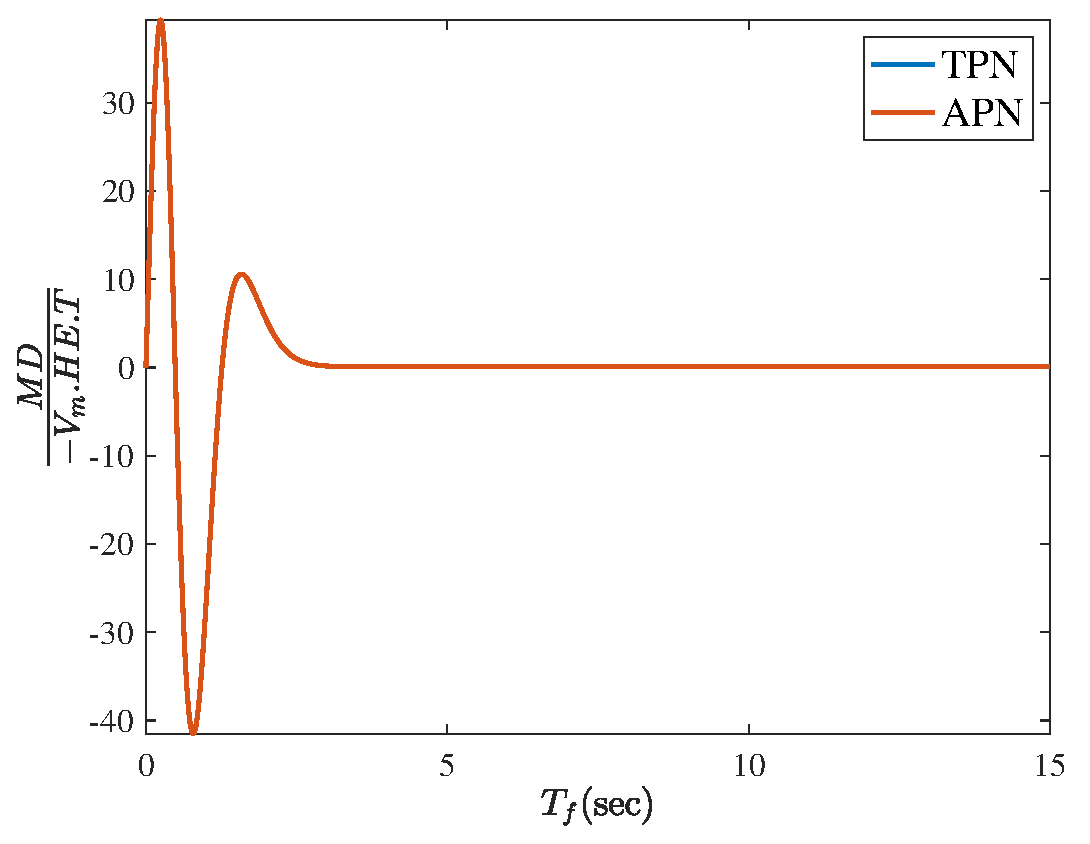
\includegraphics[width=.75\linewidth]{../Figure/Q2/c/HE_25}
	\caption{مقایسه فاصله ازدست‌دهی در قانون هدایت تناسبی حقیقی و افزوده یرای $T=0.25$ بر حسب زمان پرواز}
\end{figure}

\begin{figure}[H]
	\centering
	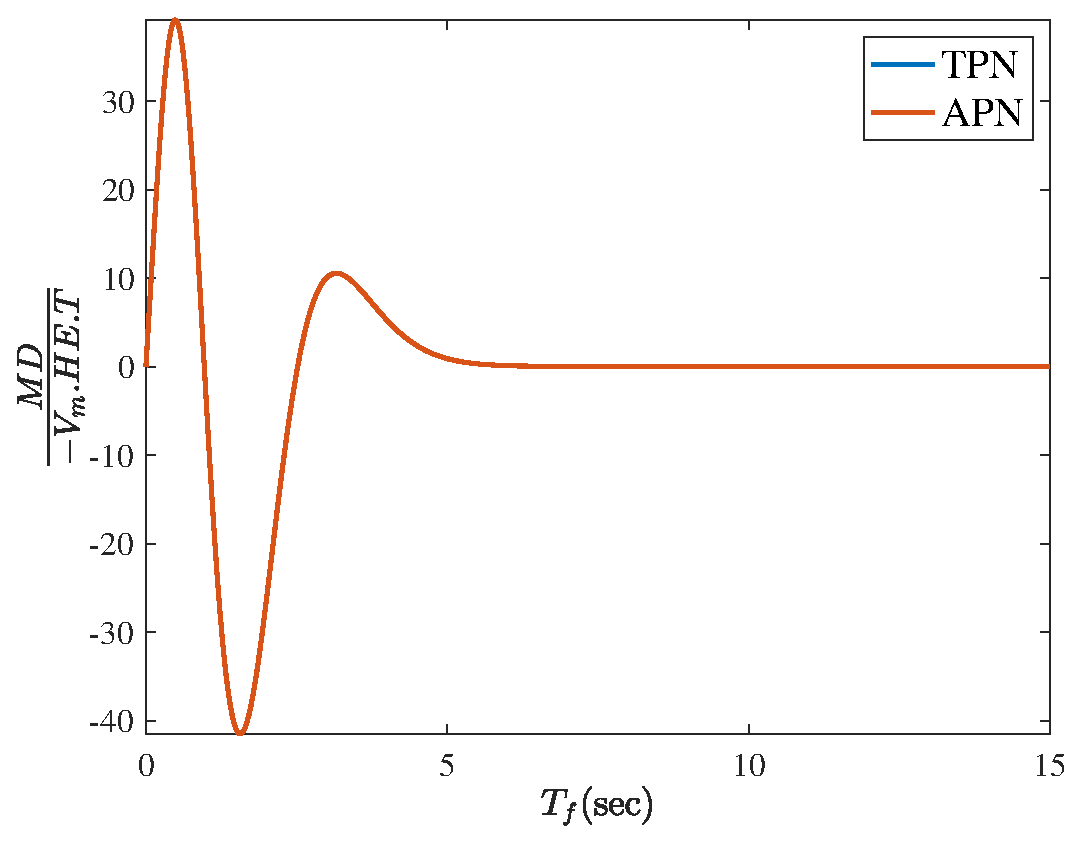
\includegraphics[width=.75\linewidth]{../Figure/Q2/c/HE_5}
	\caption{مقایسه فاصله ازدست‌دهی در قانون هدایت تناسبی حقیقی و افزوده یرای $T=0.5$ بر حسب زمان پرواز}
\end{figure}

\begin{figure}[H]
	\centering
	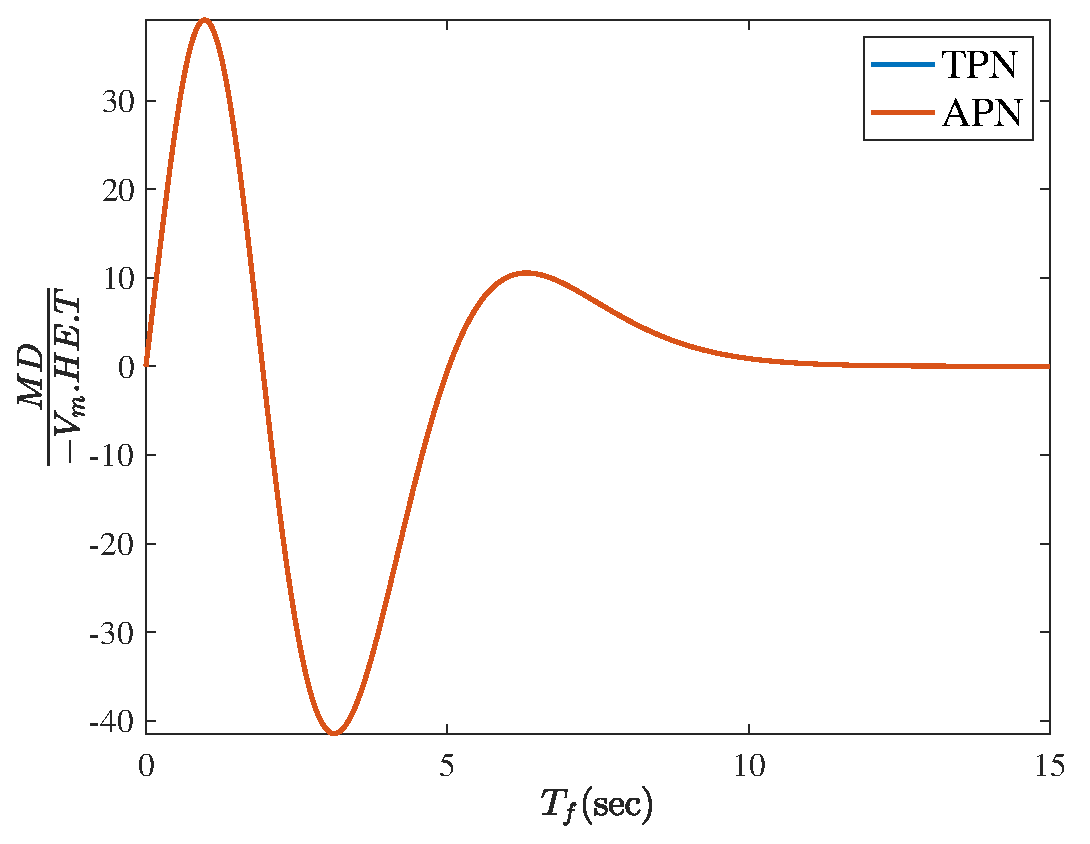
\includegraphics[width=.75\linewidth]{../Figure/Q2/c/HE_1}
	\caption{مقایسه فاصله ازدست‌دهی در قانون هدایت تناسبی حقیقی و افزوده یرای $T=1$ بر حسب زمان پرواز}
\end{figure}